\documentclass[9pt]{beamer}

%% Pre-amble - commonly defined macros.

%% Packages
\usepackage{amsmath}
\usepackage{amsfonts}
\usepackage{amssymb}
\usepackage{amsbsy}
\usepackage{isomath}
\usepackage{amsthm}
\usepackage{dsfont}
%%\usepackage{theorem}
\usepackage{algorithm}
\usepackage{algorithmicx}
\usepackage{algpseudocode}
\usepackage{mathrsfs}
\usepackage{epsfig}
\usepackage{subcaption}
\usepackage{makeidx} 
\usepackage{colortbl}
\usepackage{enumerate}
\usepackage{multirow}
\usepackage{listings}
\usepackage{pgfplots}
\newlength\fheight
\newlength\fwidth
\only<presentation>{
\setlength\fheight{0.5\columnwidth}
\setlength\fwidth{0.5\columnwidth}
}
\only<article>{
\setlength\fheight{0.25\textwidth}
\setlength\fwidth{0.25\textwidth}
}
\usepackage[sort&compress,comma,super]{natbib}
\def\newblock{} % To avoid a compilation error about a function \newblock undefined
\usepackage{hyperref}

\setbeamertemplate{theorems}[numbered] 
\mode<presentation>{
\theoremstyle{plain}
\newtheorem{assumption}{Assumption}
\theoremstyle{definition}
\newtheorem{exercise}{Exercise}
\theoremstyle{remark}
\newtheorem{remark}{Remark}
}

\numberwithin{equation}{section} 
\mode<article>{
\theoremstyle{plain}
%    \newtheorem{assumption}{Assumption}[section]
\newtheorem{lemma}{Lemma}[section]
\newtheorem{theorem}{Theorem}[section]
\newtheorem{corollary}{Corollary}[section]
\theoremstyle{definition}
\newtheorem{definition}{Definition}[section]
\theoremstyle{remark}
\newtheorem{remark}{Remark}[section]

%\theoremstyle{plain} \newtheorem{remark}{Remark}[section]
%\theoremstyle{plain} \newtheorem{definition}{Definition}[section]
\theoremstyle{plain} \newtheorem{assumption}{Assumption}[section]

%%% Examples %%%%
\newtheoremstyle{example}  % Name
{1em}       % Space above 
{1em}       % Space below
{\small}      % Body font
{}          % Indent amount 
{\scshape}  % Theorem head font
{.}         % Punctuation after theorem head
{.5em}      % Space after theorem head
{}          % Theorem head spec
\theoremstyle{example}
\newtheorem{example}{Example}
\newtheorem{exercise}{Exercise}

\usepackage{framed}
\renewenvironment{block}[1]
{\framed \par \textbf{#1} \newline}
{\par \endframed}

\renewenvironment{exampleblock}[1]
{\framed \par \textit{#1} \newline \bigskip}
{\par \endframed}

\renewenvironment{alertblock}[1]
{\framed \par \textit{\textbf{#1}} \newline \hrule \bigskip}
{\par \endframed}
}


%\theoremstyle{plain} \newtheorem{conjecture}{Conjecture}[section]
%\theoremstyle{plain} \newtheorem{theorem}{Theorem}[section]
%\theoremstyle{plain} \newtheorem{proposition}{Proposition}[section]
%\theoremstyle{plain} \newtheorem{lemma}{Lemma}[section]
%\theoremstyle{plain} \newtheorem{corollary}{Corollary}[section]


%\newenvironment{proof}[1][Proof]{\begin{trivlist}
%\item[\hskip \labelsep {\bfseries #1}]}{\end{trivlist}}
%\newcommand{\qed}{\nobreak \ifvmode \relax \else
%      \ifdim\lastskip<1.5em \hskip-\lastskip
%      \hskip1.5em plus0em minus0.5em \fi \nobreak
%      \vrule height0.5em width0.5em depth0.25em\fi}

\newcommand \indexmargin[1] {\marginpar{\emph{#1}}\index{#1}}
\newcommand \marginref[2] {\marginpar{\emph{#1}}\emph{#1}\index{#2}}
\newcommand \emindex[1] {\emph{#1}\marginpar{\emph{#1}}\index{#1}}


\newcommand \E {\mathop{\mbox{\ensuremath{\mathbb{E}}}}\nolimits}
\newcommand \hE {\hat{\mathop{\mbox{\ensuremath{\mathbb{E}}}}\nolimits}}
\renewcommand \Pr {\mathop{\mbox{\ensuremath{\mathbb{P}}}}\nolimits}
\newcommand \given {\mathrel{|}}
\newcommand \gvn {|}
\newcommand \eq {{=}}


%% Special characters
\newcommand\Reals {{\mathbb{R}}}
\newcommand\Naturals {{\mathbb{N}}} 
\newcommand\Simplex {\mathbold{\Delta}}

\newcommand \FB {{\mathfrak{B}}}
\newcommand \FD {{\mathfrak{D}}}
\newcommand \FF {{\mathfrak{F}}}
\newcommand \FM {{\mathfrak{M}}}
\newcommand \FK {{\mathfrak{K}}}
\newcommand \FJ {{\mathfrak{J}}}
\newcommand \FL {{\mathfrak{L}}}
\newcommand \FO {{\mathfrak{O}}}
\newcommand \FS {{\mathfrak{S}}}
\newcommand \FT {{\mathfrak{T}}}
\newcommand \FP {{\mathfrak{P}}}
\newcommand \FR {{\mathfrak{R}}}


\newcommand \CA {{\mathcal{A}}}
\newcommand \CB {{\mathcal{B}}}
\newcommand \CC {{\mathcal{C}}}
\newcommand \CD {{\mathcal{D}}}
\newcommand \CE {{\mathcal{E}}}
\newcommand \CF {{\mathcal{F}}}
\newcommand \CG {{\mathcal{G}}}
\newcommand \CH {{\mathcal{H}}}
\newcommand \CJ {{\mathcal{J}}}
\newcommand \CL {{\mathcal{L}}}
\newcommand \CM {{\mathcal{M}}}
\newcommand \CN {{\mathcal{N}}}
\newcommand \CO {{\mathcal{O}}}
\newcommand \CP {{\mathcal{P}}}
\newcommand \CQ {{\mathcal{Q}}}
\newcommand \CR {{\mathcal{R}}}
\newcommand \CS {{\mathcal{S}}}
\newcommand \CT {{\mathcal{T}}}
\newcommand \CU {{\mathcal{U}}}
\newcommand \CV {{\mathcal{V}}}
\newcommand \CW {{\mathcal{W}}}
\newcommand \CX {{\mathcal{X}}}
\newcommand \CY {{\mathcal{Y}}}
\newcommand \CZ {{\mathcal{Z}}}

\newcommand \BA {{\mathbb{A}}}
\newcommand \BI {{\mathbb{I}}}
\newcommand \BS {{\mathbb{S}}}

\newcommand \bx {{\mathbf{x}}}
\newcommand \by {{\mathbf{y}}}
\newcommand \bu {{\mathbf{u}}}
\newcommand \bw {{\mathbf{w}}}
\newcommand \ba {{\mathbf{a}}}
\newcommand \bz {{\mathbf{z}}}
\newcommand \bat {{\mathbf{a}_t}}
\newcommand \bh {{\mathbf{h}}}
\newcommand \bo {{\mathbf{o}}}
\newcommand \bp {{\mathbf{p}}}
\newcommand \bs {{\mathbf{s}}}
\newcommand \br {{\mathbf{r}}}

\newcommand \SA {\mathscr{A}}
\newcommand \SB {\mathscr{B}}
\newcommand \SC {\mathscr{C}}
\newcommand \SF {\mathscr{F}}
\newcommand \SG {\mathscr{G}}
\newcommand \SH {\mathscr{H}}
\newcommand \SJ {\mathscr{J}}
\newcommand \SL {\mathscr{L}}
\newcommand \SP {\mathscr{P}}
\newcommand \SR {\mathscr{R}}
%%\newcommand \SS {\mathscr{S}}
\newcommand \ST {\mathscr{T}}
\newcommand \SU {\mathscr{U}}
\newcommand \SV {\mathscr{V}}
\newcommand \SW {\mathscr{W}}

\newcommand \hM {\widehat{M}}

\newcommand \KL[2] {\mathbb{D}\left( #1 \| #2 \right)}


%\newcommand \p {\partial}

\newcommand \then{\Rightarrow}
\newcommand \defn {\mathrel{\triangleq}}
%\newcommand \StateSet {{\CQ}}


%% Commands

\newcommand \argmax{\mathop{\rm arg\,max}}
\newcommand \argmin{\mathop{\rm arg\,min}}
\newcommand \dtan{\mathop{\rm dtan}}
\newcommand \sgn{\mathop{\rm sgn}}
\newcommand \trace{\mathop{\rm tr}}

\newcommand \onenorm[1]{\left\|#1\right\|_1}
\newcommand \pnorm[2]{\left\|#1\right\|_{#2}}
\newcommand \inftynorm[1]{\left\right\|#1\|_\infty}
\newcommand \norm[1]{\left\|#1\right\|}

%%\newcommand \defn {\triangleq}
%%\newcommand \defn {\equiv}
%%\newcommand \defn {\coloneq}
%%\newcommand \defn {\stackrel{\text{\tiny def}}{=}}
%%\newcommand \defn {\stackrel{\text{def}}{\hbox{\equalsfill}}}

\DeclareMathAlphabet{\mathpzc}{OT1}{pzc}{m}{it}

\newcommand \Normal {\mathop{\mathpzc{N}}\nolimits}
\newcommand \Poisson {\mathop{\mathpzc{Poisson}}\nolimits}
\newcommand \Multinomial {\mathop{\mathpzc{Multinomial}}\nolimits}
\newcommand \Dirichlet {\mathop{\mathpzc{Dirichlet}}\nolimits}
\newcommand \Student {\mathop{\mathpzc{Student}}\nolimits}
\newcommand \Bernoulli {\mathop{\mathpzc{Bernoulli}}\nolimits}
\newcommand \BetaDist   {\mathop{\mathpzc{Beta}}\nolimits}
\newcommand \Singular   {\mathop{\mathpzc{D}}\nolimits}
\newcommand \GammaDist {\mathop{\mathpzc{Gamma}}\nolimits}
\newcommand \Softmax{\mathop{\mathpzc{Softmax}}\nolimits}
\newcommand \Exp{\mathop{\mathpzc{Exp}}\nolimits}
\newcommand \Uniform{\mathop{\mathpzc{Unif}}\nolimits}
\newcommand \Laplace {\mathop{\mathpzc{Laplace}}\nolimits}

\newcommand \Param {\Theta}
\newcommand \param {\theta}
\newcommand \vparam {\vectorsym{\theta}}
\newcommand \mparam {\matrixsym{\Theta}}
\newcommand \Hyperparam {\Phi}
\newcommand \hyperparam {\phi}
\newcommand \family {\mathcal{F}}
\newcommand{\ie}{\emph{i.e.}\xspace}
\newcommand{\eg}{\emph{e.g.}\xspace}
\newcommand{\etal}{\emph{et al.}\xspace}
\newcommand{\constg}{}
\newcommand{\Bel}{\Xi}
\newcommand \Bay {\ensuremath{\mathscr{B}}}
\newcommand \Adv {\ensuremath{\mathscr{A}}}


\newcommand \Borel[1] {\FF(#1)}
\newcommand \Probs[1] {\FM(#1)}


\newcommand \pol {\pi}
\newcommand \Pol {\Pi}
\newcommand \mdp {\mu}
\newcommand \MDP {\CM}
\newcommand \meanMDP {{\bar{\mdp}_\xi}}

\newcommand {\msqr} {\vrule height0.33cm width0.44cm}
\newcommand {\bsqr} {\vrule height0.55cm width0.66cm}

\newcommand\ind[1]{\mathop{\mbox{\ensuremath{\mathbb{I}}}}\left\{#1\right\}}
\newcommand\Ind{\mbox{\bf{I}}}

\newcommand\dd{\,\mathrm{d}}

\newcommand \seq[2]{#1^{#2}}
\newcommand \pseq[3]{#1_{#2}^{#3}}
\newcommand \sam[2]{#1^{(#2)}}
\newcommand \transpose[1] {#1^\top}
\newcommand\set[1] {\left\{#1\right\}}
\newcommand\tuple[1] {\left\langle #1\right\rangle}
\newcommand\cset[2] {\left\{#1 ~\middle|~ #2\right\}}
\newcommand \ceil[1]{\left\lceil #1 \right\rceil}





\newcommand{\indep}{\mathrel{\text{\scalebox{1.07}{$\perp\mkern-10mu\perp$}}}}


\newcommand \eqlike {\eqsim}
\newcommand \gtlike {\succ}
\newcommand \ltlike {\prec}
\newcommand \gelike {\succsim}
\newcommand \lelike {\precsim}

\newcommand \eqpref {\eqsim^*}
\newcommand \gtpref {\succ^*}
\newcommand \ltpref {\prec^*}
\newcommand \gepref {\succsim^*}
\newcommand \lepref {\precsim^*}

\newcommand \util {U}
\newcommand \BUtil {U^*}
\newcommand \MUtil {\matrixsym{U}}
\newcommand \risk {\sigma}
\newcommand \Brisk {\sigma^*}
\newcommand \Loss {\ell}
\newcommand \Regret {L}
\newcommand \regret {\ell}
\newcommand \Reward {\SR}
\newcommand \reward {r}
\newcommand \vreward {\vectorsym{r}}
\newcommand \Rew {\rho}
\newcommand \outcome {\omega}
\newcommand \Outcome {\Omega}
\newcommand \act {a}
\newcommand \Act {\CA}
\newcommand \decision {a}
\newcommand \Decision {\mathcal{A}}
\newcommand \dec {\delta}
\newcommand \Dec {\mathscr{D}}


\newcommand {\MH} {\matrixsym{H}}

\newcommand \alg {\lambda}
\newcommand \Alg {\Lambda}
\newcommand \KNN {\textsc{k-NN}}

\newcommand \model {\mu}
\newcommand \MAP {\model_{\textrm{MAP}}}
\newcommand \Model {\CM}
\newcommand \Datasets {\CD}
\newcommand \Data {D}
\newcommand \Training {D_T}
\newcommand \Holdout {D_H}
\newcommand \Testing {D^*}
\newcommand \error {\epsilon}
\newcommand \obs {x}
\newcommand \Obs {\CX}
\newcommand \Att {\CA}
\newcommand \att {a}
\newcommand \attv {v}
\newcommand \Attv {\CV}
\newcommand \cls {y}
\newcommand \Cls {\CY}
\newcommand \Entropy {\mathbb{H}}
\newcommand \Gain {\mathbb{G}}


\newcommand \IDThree {\texttt{ID3}}

\newcommand \nactions {A}
\newcommand \nclasses {C}
\newcommand \nstates{S}
\newcommand \nobservations {N}
\newcommand \ndata{T}

\newcommand \figwidth {0.6\textwidth}
\newcommand \figheight {0.4\textwidth}

\newcommand \eye {\matrixsym{I}}
\newcommand \MA {\matrixsym{A}}
\newcommand \MX {\matrixsym{X}}
\newcommand \MY {\matrixsym{Y}}
\newcommand \MB {\matrixsym{B}}
\newcommand \MV {\matrixsym{V}}
\newcommand \MW {\matrixsym{W}}
\newcommand \MP {\matrixsym{P}}
\newcommand \vg {\vectorsym{\gamma}}
\newcommand \vp {\vectorsym{p}}
\newcommand \vs {\vectorsym{s}}
\newcommand \vx {\vectorsym{x}}
\newcommand \vr {\vectorsym{r}}
\newcommand \vm {\vectorsym{m}}
\newcommand \vb {\vectorsym{b}}
\newcommand \vt {\vectorsym{\theta}}

\newcommand \pn[1] {\vx_{[#1]}}

\newcommand \basis {f}
\newcommand \bel {\xi}
\newcommand \hyper {\omega}
\newcommand \mbel {\bel^D}
\newcommand \pbel {\bel^C}

\newcommand \pmean {\matrixsym{M}}
\newcommand \pcov {\matrixsym{C}}
\newcommand \pwish {\matrixsym{W}}
\newcommand \porder {n}

\newcommand \Syx {\matrixsym{\Sigma}_{yx}}
\newcommand \Sxx {\matrixsym{\Sigma}_{xx}}
\newcommand \Syy {\matrixsym{\Sigma}_{yy}}
\newcommand \Symx {\matrixsym{\Sigma}_{y\mid x}}

\newcommand \trans {\matrixsym{P}}
\newcommand \ident {\matrixsym{I}}

\newcommand \noise {\vectorsym{\varepsilon}}

\newcommand \pt {p_t}


\newcommand \CSet {G}
\newcommand \Parent[1] {\mathfrak{P}(#1)}
\newcommand \Children[1] {\mathfrak{C}(#1)}
\newcommand \Ancestors[1] {\mathfrak{A}(#1)}
\newcommand \Descendants[1] {\mathfrak{D}(#1)}
\newcommand \metric[2] {\nu(#1, #2)}
\newcommand \zooming {\zeta}
\newcommand \depth[1] {d(#1)}

\newcommand \sensitivity[1] {\mathbb{L}\left(#1\right)}
\newcommand \disc {\gamma}
\newcommand \Value {V}
\newcommand \val {\vectorsym{v}}
\newcommand \Vals {\mathcal{V}}
\newcommand \qval {\vectorsym{q}}
\newcommand \Qvals {\mathcal{Q}}
\newcommand \blm {\mathscr{L}}
\newcommand \tdm {\mathscr{D}}
\newcommand \pim {\mathscr{B}}



\newcommand \dist[2]{D\left(#1 ~\middle\|~ #2\right)}

\newcommand \Ae {A_\epsilon^\hist}

\newcommand \lrdist[2]{d_{lr}(#1, #2)}
\newcommand \xdistChar{\rho}
\newcommand \xdist[2]{\xdistChar(#1, #2)}
\newcommand \pdist[2]{\kappa(#1, #2)}
\newcommand{\constScale}{\omega}
\newcommand{\constScaleB}{\kappa}

\newcommand \fields[1]{\sigma(#1)}

\newcommand \hist {h}

\newcommand \abs[1] {\left|#1\right|}

\newcommand{\errorband}[5][]{ % x column, y column, error column, optional argument for setting style of the area plot
\pgfplotstableread[col sep=comma, skip first n=2]{#2}\datatable
% Lower bound (invisible plot)
\addplot [draw=none, stack plots=y, forget plot] table [
x={#3},
y expr=\thisrow{#4}-\thisrow{#5}
] {\datatable};

% Stack twice the error, draw as area plot
\addplot [draw=none, fill=gray!40, stack plots=y, area legend, #1] table [
x={#3},
y expr=2*\thisrow{#5}
] {\datatable} \closedcycle;

% Reset stack using invisible plot
\addplot [forget plot, stack plots=y,draw=none] table [x={#3}, y expr=-(\thisrow{#4}+\thisrow{#5})] {\datatable};
}


%%% macros to make things smalller
% For comparison, the existing overlap macros:
% \def\llap#1{\hbox to 0pt{\hss#1}}
% \def\rlap#1{\hbox to 0pt{#1\hss}}
\def\clap#1{\hbox to 0pt{\hss#1\hss}}
\def\mathllap{\mathpalette\mathllapinternal}
\def\mathrlap{\mathpalette\mathrlapinternal}
\def\mathclap{\mathpalette\mathclapinternal}
\def\mathllapinternal#1#2{%
\llap{$\mathsurround=0pt#1{#2}$}}
\def\mathrlapinternal#1#2{%
\rlap{$\mathsurround=0pt#1{#2}$}}
\def\mathclapinternal#1#2{%
\clap{$\mathsurround=0pt#1{#2}$}}


\usepackage{tikz}

%\usetikzlibrary{external}
%\tikzexternalize[prefix=tikz/]
\usepackage{gnuplot-lua-tikz}


\usetikzlibrary{automata}
\usetikzlibrary{topaths}
\usetikzlibrary{shapes}
\usetikzlibrary{arrows}
\usetikzlibrary{decorations.markings}
\usetikzlibrary{intersections}
\usetikzlibrary{backgrounds}


\tikzstyle{utility}=[diamond,draw=black,draw=blue!50,fill=blue!10,inner sep=0mm, minimum size=8mm]
\tikzstyle{select}=[rectangle,draw=black,draw=blue!50,fill=blue!10,inner sep=0mm, minimum size=6mm]
\tikzstyle{hidden}=[dashed,draw=black,fill=red!10]
\tikzstyle{RV}=[circle,draw=black,draw=blue!50,fill=blue!10,inner sep=0mm, minimum size=6mm]
\tikzstyle{place}=[circle,draw=black,draw=blue!50,fill=blue!20,inner sep=0mm, minimum size=9mm]
\tikzstyle{select}=[rectangle,draw=black,draw=blue!50,fill=blue!20,inner sep=0mm, minimum size=6mm]
\tikzstyle{transition}=[rectangle,draw=black!50,fill=black!20,thick]
\tikzstyle{observed}=[circle,draw=black,draw=blue!50,fill=blue!10,inner sep=0mm, minimum size=6mm]
\tikzstyle{someset}=[circle,draw=black,minimum size=8mm]

\tikzstyle{known}=[rectangle,draw=green!50,fill=green!20,thick]
\tikzstyle{queried}=[rectangle,draw=blue!50,fill=blue!20,thick]
%\tikzstyle{transition}=[rectangle,draw=black!50,fill=black!20,thick]

\tikzstyle{thickarrow}=[->, >=latex, line width=15pt, green!50]
\tikzstyle{medarrow}=[->, >=latex,  line width=5pt]
\tikzstyle{arrow}=[->,>=triangle 60]

\tikzset{every picture/.style={
    line width=1
  }
}

\definecolor{dark-green}{rgb}{0,0.5,0}



%\usepackage{pstool}
\usepackage{listings}
\usepackage{overpic}
\title{Experiment design}
\subtitle{Bandit problems and Markov decision processes}
\author{Christos Dimitrakakis}
\institute{UiO}

%% \logo{\includegraphics[height=0.5cm]{cit_logo.png}}

%%%%%%%%%%%%%%%%%%%%%%%%%%%%%%%%%%% Colors %%%%%%%%%%%%%%%%%%%%%%%%%%%%%%%%%%%%%
\newcommand{\InBlue}{\color{blue}}
\newcommand{\InGreen}{\color{green}}
%%%%%%%%%%%%%%%%%%%%%%%%%%%%%%%%%%%%%%%%%%%%%%%%%%%%%%%%%%%% 
\begin{document}


\begin{frame}
  \titlepage
\end{frame}

\begin{frame}
  \tableofcontents
\end{frame}



\begin{frame}
  \frametitle{Sequential problems: full observation}
  \begin{example}
    \begin{itemize}
    \item $n$ meteorological stations $\cset{\mdp_i}{i=1, \ldots,n}$
    \item The $i$-th station gives a rain probability $x_{t,i} = P_{\mdp_i}(y_t \mid y_1, \ldots, y_{t-1})$.
    \end{itemize}
  \end{example}
  \begin{itemize}
  \item Observation $\bx_t = (x_{t,1}, \ldots, x_{t,n})$: the predictions of all stations.
  \item Decision $\decision_t$: Guess if it will rain
  \item Outcome $y_t$: Rain or not rain.
  \item Steps $t = 1, \ldots, T$.
  \end{itemize}

  \begin{block}{Linear utility function}
    Reward function is $\Rew(y_t, a_t) = \ind{y_t = a_t}$ simply rewarding correct predictions with utility being
    \[
      U(y_1, y_2, \ldots, y_T, \decision_1, \ldots, \decision_T)
      = 
      \sum_{t=1}^T \Rew(y_t, \decision_t),
    \]
    the total number of correct predictions.
  \end{block}

\end{frame}


\section{Bandit problems}
\label{sec:exp-design-bandit}

\begin{frame}

  The $n$ meteorologists problem is simple, as:

  \begin{itemize}
  \item You always see their predictions, as well as the weather, no matter whether you bike or take the tram (full information)
  \item Your actions do not influence their predictions (independence events)
  \end{itemize}
  
  In the remainder, we'll see two settings where decisions are made with either \alert{partial information} or in a \alert{dynamical system}. Both of these settings can be formalised with Markov decision processes.

\end{frame}



\only<presentation>
{
  \begin{frame}\frametitle{Experimental design and Markov decision processes}
    The following problems
    \begin{itemize}
    \item Shortest path problems.
    \item Optimal stopping problems.
    \item Reinforcement learning problems.
    \item Experiment design (clinical trial) problems
    \item Advertising. \only<article>{This was first real-world application of Markov decision processes. In fact, Howard used the formalism when he was a graduate student in order to find an optimal advertising catalog mailing policy based on customers' purchasing behaviour.}
    \end{itemize}
    can be all formalised as \alert{Markov decision processes}.

    \begin{block}{Applications}
      \begin{itemize}
      \item Robotics.
      \item Economics.
      \item Automatic control.
      \item Resource allocation
      \end{itemize}
    \end{block}
  \end{frame}
}


\begin{frame}
  \frametitle{Bandit problems}
  \only<1>{ 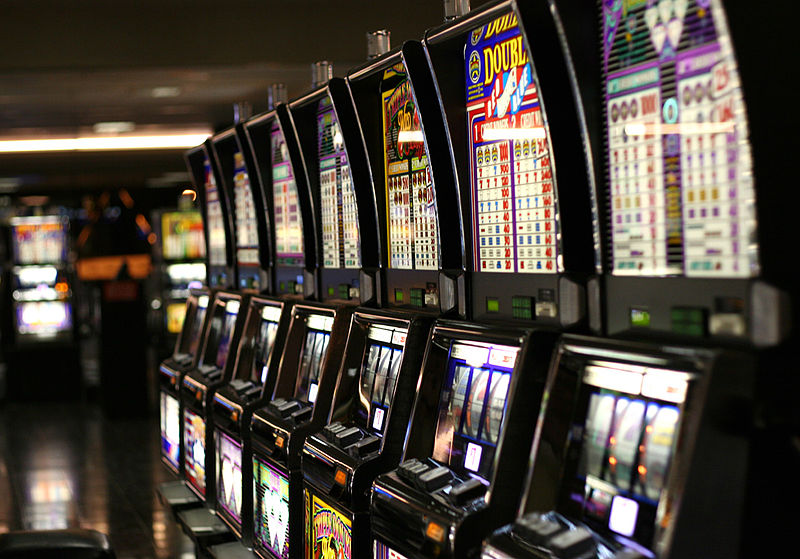
\includegraphics[width=\textwidth]{../figures/Las_Vegas_slot_machines}
  }
  \only<2->{
    \begin{columns}
      \begin{column}{0.6\textwidth}
        \begin{block}{Applications}
          \begin{itemize}
          \item<2-> Efficient optimisation.
          \item<3-> Online advertising.
          \item<4-> Clinical trials.
          \item<5-> \textsc{Robot scientist}.
          \end{itemize}
        \end{block}
      \end{column}
      \begin{column}{0.4\textwidth}
        \only<2>{
          \begin{tikzpicture}[domain=0:10]
            \draw[very thin,color=gray] (-0.1,-1.1) grid (2.9,2.9);
            \draw[->] (-0.2,0) -- (3.2,0) node[right] {$x$};
            \draw[->] (0,-1.2) -- (0,3.2) node[above] {$f(x)$};
            \draw[color=blue] plot (\x / 5,{sin(10 \x r)/(1 + \x)}) node[above] {$f(x) = \mathrm{sinc} x$};
          \end{tikzpicture}
        }             \only<3>{
\includegraphics[width=0.8\textwidth]{../figures/google-logo}}

        \only<4>{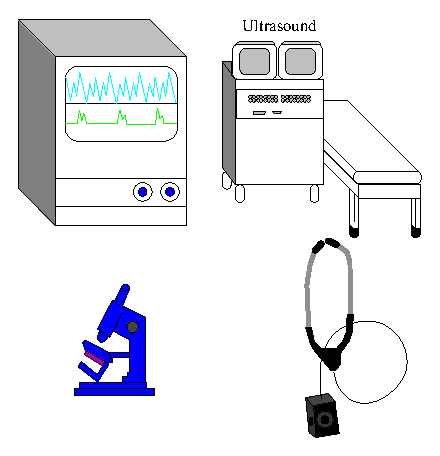
\includegraphics[width=0.8\textwidth]{../figures/clinical}}
        \only<5>{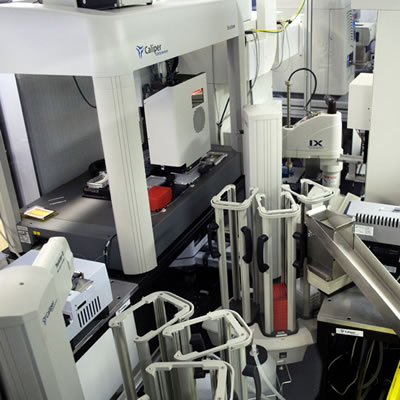
\includegraphics[width=0.8\textwidth]{../figures/robot-scientist}}
      \end{column}
    \end{columns}
  }
\end{frame}


\begin{frame}  
  \frametitle{The stochastic $n$-armed bandit problem}
  \begin{block}{Actions and rewards}
    \begin{itemize}
    \item A set of \alert{actions} $\CA = \set{1, \ldots, n}$.
    \item Each action gives you a \alert{random reward} with distribution $\Pr(r_t \mid a_t = i)$.
    \item The  \alert{expected reward} of the $i$-th arm is $\rho_i \defn \E(r_t \mid a_t = i)$.
    \end{itemize}
  \end{block}
  \begin{exampleblock}{Interaction at time $t$}
    \begin{enumerate}
    \item You choose an action $a_t \in \CA$.
    \item You observe a random reward $r_t$ drawn from the $i$-th arm.
    \end{enumerate}
  \end{exampleblock}
  \begin{block}{The utility is the \alert{sum of the rewards} obtained}
    \[
      U \defn \sum_{t} r_t.
    \]
  \end{block}
  We must maximise the expected utility, \alert{without knowing} the values $\rho_i$.
\end{frame}

\begin{frame}
  \frametitle{Policy}
  \begin{definition}[Policies]
    A policy $\pol$ is \alert{an algorithm for taking actions} given the observed history $h_t \defn a_1, r_1, \ldots, a_t, r_t$
    \[
      \Pr^\pol(a_{t+1} \mid h_t)
    \]
    is the probability of the next action $a_{t+1}$.
  \end{definition}
  \only<1>{
    \begin{exercise}
      Why should our action depend on the complete history?
      \begin{itemize}
      \item[A] The next reward depends on all the actions we have taken.
      \item[B] We don't know which arm gives the highest reward.
      \item[C] The next reward depends on all the previous rewards.
      \item[D] The next reward depends on the complete history.
      \item[E] No idea.
      \end{itemize}
    \end{exercise}}
  \only<2-3>{
    \begin{example}[The expected utility of a uniformly random policy]
      If $\Pr^\pol(a_{t+1} \mid \cdot) = 1/n$ for all $t$, then
      \only<3>{
        \[
          \E^\pol U = \E^\pol \left(\sum_{t=1}^T r_t \right)
          = \sum_{t=1}^T \E^\pol r_t
          = \sum_{t=1}^T \sum_{i=1}^n \frac{1}{n} \rho_i
          = \frac{T}{n} \sum_{i=1}^n \rho_i
        \]
      }
    \end{example}
  }
  \only<4->{
    \begin{block}{The expected utility of a general policy}
      \begin{align}
        \onslide<4->{\E^\pol U &= \E^\pol \left(\sum_{t=1}^T r_t \right) }
                                 \onslide<5->{ = \sum_{t=1}^T \E^\pol(r_t)\\ }
        \onslide<6->{
                               & = \sum_{t=1}^T  \sum_{a_t \in \CA}  \E (r_t \mid a_t) 
                                 \sum_{h_{t-1}}
                                 \Pr^\pol(a_t \mid h_{t-1})
                                 \Pr^\pol(h_{t-1})
                                 }
                                 \notag
      \end{align}
    \end{block}
  }


\end{frame}



\subsection{Planning: Heuristics and exact solutions}
\label{sec:exp-design-bandit}
\index{bandit problems}


\begin{frame}
  \frametitle{A simple heuristic for the unknown reward case}
  Say you keep a \alert{running average} of the reward obtained by each arm
  \[
  \hat{\param}_{t,i} = R_{t,i} / n_{t,i}
  \]
  \begin{itemize}
  \item $n_{t,i}$ the number of times you played arm $i$ 
  \item $R_{t,i}$ the total reward received from $i$.
  \end{itemize}
  Whenever you play $a_t = i$:
  \[
  R_{t+1, i} = R_{t,i} + r_t, \qquad n_{t+1,i} = n_{t,i} + 1.
  \]
  Greedy policy:
  \[
  a_t = \argmax_i \hat{\param}_{t,i}.
  \]
  What should the initial values $n_{0,i}, R_{0,i}$ be?
\end{frame}


\begin{frame}
  \frametitle{Bernoulli bandits}
  \begin{block}{Decision-theoretic approach}
    \begin{itemize}
    \item Assume $r_t \mid a_t = i \sim P_{\param_i}$, with $\param_i\in \Param$.
    \item Define prior belief  $\xi_1$ on $\Param$.
    \item For each step $t$, find a policy $\pol$ selecting action $a_t \mid \bel_t \sim \pol(a \mid \bel_t)$ to 
      \[
      \max_\pol \E^\pol_{\xi_t}(U_t) = \max_\pol \E^\pol_{\xi_t} \sum_{a_t} \left(\sum_{k=1}^{T-t}  r_{t+k} ~\middle|~ a_t \right) \pol(a_t \mid \bel_t).
      \]
    \item Obtain reward $r_t$.
    \item Calculate the next belief
      \[
        \xi_{t+1} = \xi_t(\cdot \mid a_t, r_t)
      \]
    \end{itemize}
  \end{block}
  How can we implement this?
\end{frame}






\begin{frame}
  \frametitle{Bayesian inference on Bernoulli bandits}
  \only<1>{
    \begin{itemize}
    \item Likelihood: $\Pr_\param(r_t = 1) = \param$.
    \item Prior: $\bel(\param) \propto \param^{\alpha - 1} (1 - \param)^{\beta - 1}$ \quad (i.e. $\BetaDist(\alpha, \beta)$).
    \end{itemize}
    \begin{figure}[h]
      \centering
      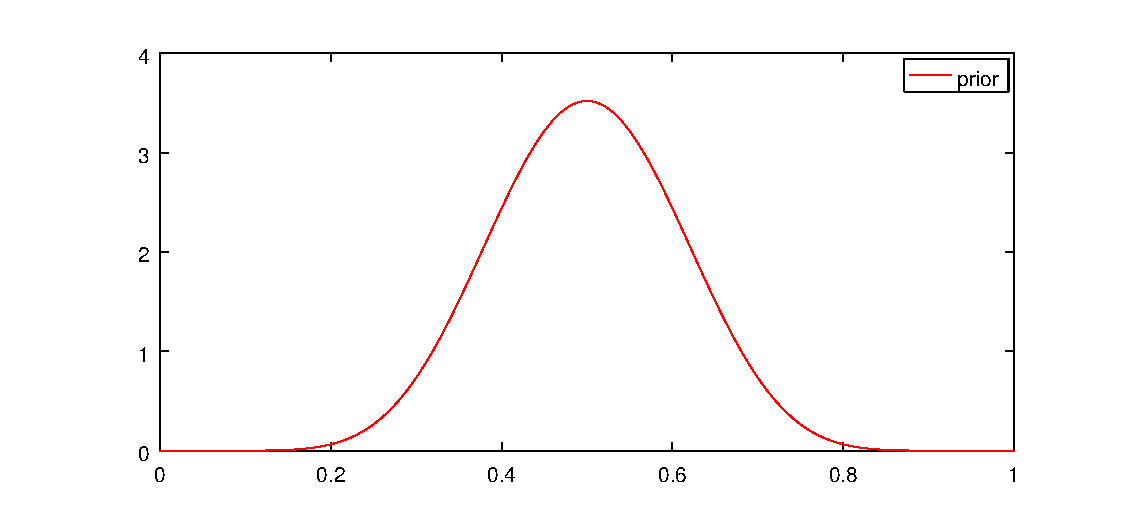
\includegraphics[width=\textwidth]{../figures/beta-prior}
      \caption{Prior belief $\bel$ about the mean reward $\param$.}
    \end{figure}
  }
  \only<2>{
    For a sequence $r = r_1, \ldots, r_n$, $\Rightarrow$
    $P_{\param}(r) \propto  \param_i^{\textrm{\#1(r)}} (1 - \param_i)^{\textrm{\#0(r)}}$

    \begin{figure}[h]
      \centering
      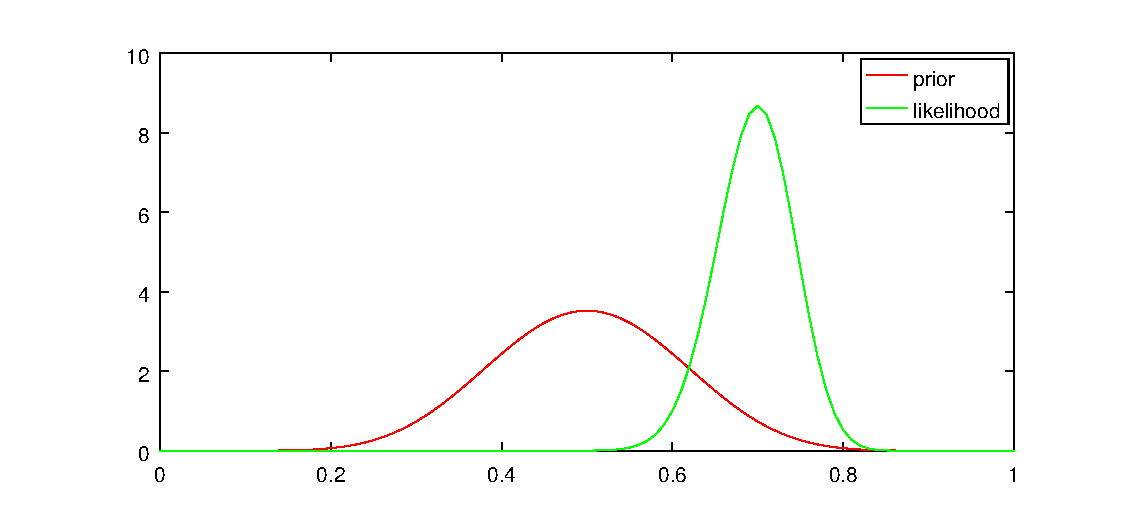
\includegraphics[width=\textwidth]{../figures/beta-likelihood}
      \caption{Prior belief $\bel$ about $\param$ and likelihood of $\param$ for 100 plays with 70 1s.}
    \end{figure}
  }
  \only<3->{
    Posterior: $\BetaDist(\alpha + \textrm{\#1(r)}, \beta + \textrm{\#0(r)})$.
    \begin{figure}[h]
      \centering
      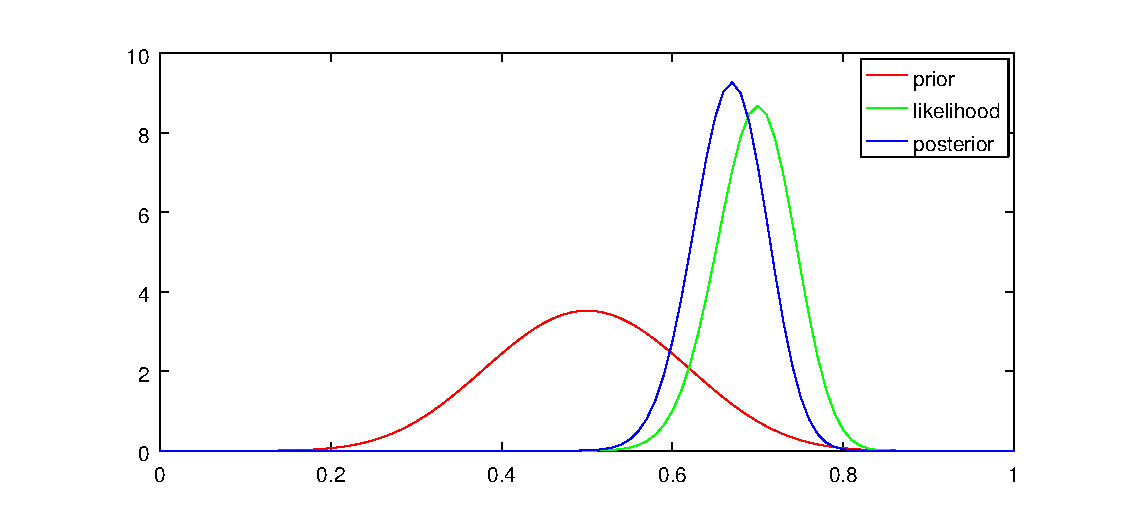
\includegraphics[width=\textwidth]{../figures/beta-posterior}
      \caption{Prior belief $\bel(\param)$ about $\param$, likelihood of $\param$ for the data $r$, and posterior belief $\bel(\param \mid r)$}
    \end{figure}
  }
\end{frame}



\begin{frame}
  \only<presentation>{\frametitle{Bernoulli example.}}
  \only<article>{As a simple illustration, consider the case when the reward for choosing one of the $n$ actions is either $0$ or $1$, with some fixed, yet unknown probability depending on the chosen action. This can be modelled in the standard Bayesian framework using the Beta-Bernoulli conjugate prior. More specifically, we can formalise the problem as follows.}

  Consider $n$ Bernoulli distributions with
  unknown parameters $\param_i$ ($i = 1, \ldots, n$) such that 
  \begin{align}
    r_t \mid a_t = i &\sim
                       \Bernoulli(\param_i),
    &
      \E(r_t  \mid a_t = i) &= \param_i.
  \end{align}
  \only<article>{Each Bernoulli distribution thus corresponds to the distribution of rewards obtained from each bandit that we can play.
    In order to apply the statistical decision theoretic framework, we have to quantify our uncertainty about the parameters $\param$ in terms of a probability distribution.
  }
  Our belief for each parameter $\param_i$ is $\BetaDist(\alpha_i,
  \beta_i)$, with density $f(\param \mid \alpha_i, \beta_i)$ so that
  \[
    \xi(\param_1, \ldots, \param_n)
    =
    \prod_{i=1}^n f(\param_i \mid \alpha_i, \beta_i).
    \tag{a priori independent}
  \]
  \[
    N_{t,i} \defn \sum_{k=1}^t \ind{a_k = i}, \qquad
    \hat{r}_{t,i} \defn \frac{1}{N_{t,i}} \sum_{k=1}^t r_t \ind{a_k = i}
  \]
  Then, the posterior distribution for the parameter of arm $i$ is
  \[
    \xi_t  = \BetaDist(\alpha^t_i, \beta^t_i),
    \qquad
    \alpha^t_i = \alpha_i + N_{t,i} \hat{r}_{t,i}~,~ \beta^t_i = \beta_i N_{t,i} (1 - \hat{r}_{t,i})).
  \]
  Since $r_t \in \{0,1\}$ there are \alert{$O((2n)^T)$ possible belief states} for a $T$-step bandit problem.
\end{frame}



\only<presentation>{
  \begin{frame}
    \frametitle{Belief states}
    \begin{itemize}
    \item The state of the decision-theoretic bandit problem is the state of our belief.
    \item A sufficient statistic is the number of plays and total rewards.
    \item Our belief state $\bel_t$ is described by the priors
      $\alpha, \beta$ and the vectors
      
      \begin{align}
        N_t = (N_{t,1}, \ldots, N_{t,i})\\
        \hat{r}_t = (\hat{r}_{t,1}, \ldots, \hat{r}_{t,i}).
      \end{align}
    \item The next-state probabilities are defined as:
      \[
        \Pr_{\bel_t}(r_t = 1 \mid a_t = i) = \frac{\alpha^t_i}{\alpha^t_i + \beta^t_i}
      \]
      as $\bel_{t+1}$ is a deterministic function of $\bel_t$, $r_t$ and $a_t$
    \item Optimising this results in a \alert{\index{Markov decision process}Markov decision process}.
    \end{itemize}
  \end{frame}
}
\only<article>{
  The state of the bandit problem is the state of our belief.
  A sufficient statistic for our belief is the number of times
  we played each bandit and the total reward from each bandit.
  Thus, our state at time $t$ is entirely described by our priors
  $\alpha, \beta$ (the initial state) and the vectors
  \begin{align}
    N_t = (N_{t,1}, \ldots, N_{t,i})\\
    \hat{r}_t = (\hat{r}_{t,1}, \ldots, \hat{r}_{t,i}).
  \end{align}
  At any time $t$, we can calculate the probability of observing
  $r_t = 1$ or $r_t = 0$ if we pull arm $i$ as:
  \[
    \xi_t(r_t = 1 \mid a_t = i) = \frac{\alpha_i + N_{t,i} \hat{r}_{t,i}}{\alpha_i + \beta_i + N_{t,i}}
  \]
  The next state is well-defined and depends only on the current
  state. As we shall see later, this type of decision problem is called a Markov decision process. Although extremely simple, This particular bandit problem is quite large. If we have a horizon $T$, then the possible beliefs we could have when our rewards are binary are in the order of $(2n)^T$.
}  


\label{sec:decision-theoretic-bandits}
\only<article>{
  The basic bandit process can be seen in Figure~\ref{fig:basic-bandit-process}. The general decision-theoretic bandit process, not restricted to independent Bernoulli bandits, can be formalised as follows.
  \begin{definition}
    Let $\CA$ be a set of actions, not necessarily finite. Let $\Param$ be a set of possible parameter values, indexing a family of probability measures $\family = \cset{P_{\param, a}}{\param \in \Param, a \in \CA}$. There is some $\param \in \Param$ such that, whenever we take action $a_t = a$, we observe reward $r_t$ with probability measure:
    \begin{equation}
      \label{eq:bandit-reward-probability}
      P_{\param,a}(R) \defn \Pr_\param(r_{t} \in R \mid a_t = a),
      \qquad R \subseteq \Reals.
      % ro: What is R? Is R on the lhs the same as on the rhs? % cd: it's just a set
    \end{equation}
    Let $\bel_1$ be a prior distribution on $\Param$ and let the posterior distributions be defined as:
    \begin{equation}
      \label{eq:bandit-posteriors}
      \bel_{t+1}(B) \propto \int_B P_{\param, a_t} (r_t) \dd \bel_t(\param).
    \end{equation}
    The next belief is random, since it depends on the random quantity $r_t$. In fact, the probability of next rewards if $a_t = a$ is given by:
    \begin{equation}
      \label{eq:dt-bandit-reward-probability}
      P_{\bel_t, a} (R) \defn \int_\Param P_{\param,a}(R) \dd{\bel_t}(\param) %ro: What is R?
    \end{equation}
    Finally, as $\bel_{t+1}$ deterministically depends on $\bel_t, a_t, r_t$, the probability of obtaining a particular next belief is the same as the probability of obtaining the corresponding rewards leading to the next belief. In more detail, we can write:
    \begin{equation}
      \label{eq:dt-bandit-belief-probability}
      \Pr(\bel_{t+1} = \bel \mid \bel_t, a_t)
      =
      \int_\CR \ind{\bel_{t}(\cdot \mid a_t, r_t = r) = \bel} \dd{P_{\bel_t, a}}(r).  %ro: What is \CR?
    \end{equation}
  \end{definition}
  In practice, although multiple reward sequences may lead to the same beliefs, we frequently ignore that possibility for simplicity. Then the process becomes a tree. A solution to the problem of what action to select is given by a backwards induction algorithm similar to that given in Section~\ref{sec:backwards-induction}.
  \begin{equation}
    U^*(\bel_t) = \max_{a_t} \E(r_t \mid \bel_t, a_t) + \sum_{\bel_{t+1}} \Pr(\bel_{t+1} \mid \bel_t, a_t) U^*(\bel_{t+1}).\label{eq:backwards-induction-bandits}
  \end{equation}
  The above equation is the \emindex{backwards induction} algorithm for bandits.  If you look at this structure, you can see that  next belief only depends on the current belief, action and reward, i.e. it satisfies the Markov property. Consequently, a decision-theoretic bandit process can be modelled more generally as a \index{Markov decision process}Markov decision process, explained in the following section. It turns out that backwards induction, as well as other efficient algorithms, can provide optimal solutions for Markov decision processes.
}


\begin{frame}
  \frametitle{Markov process}
  \begin{figure}
    \begin{tikzpicture}
      \node[RV] (x1) {$s_{t-1}$};
      \node[RV] (x2) [right of=x1] {$s_t$};
      \node[RV] (x3) [right of=x2] {$s_{t+1}$};
      \draw [->] (x1) -- (x2);
      \draw [->] (x2) -- (x3);
    \end{tikzpicture}
  \end{figure}

  \begin{definition}[Markov Process -- or Markov Chain]
    The sequence $\cset{s_t}{t=1,\ldots}$ of random variables $s_t : \Param \to \CS$ is a Markov process if
    \begin{equation}
      \label{eq:markov-chain}
      \Pr(s_{t+1} \mid s_{t}, \ldots, s_1) 
      =
      \Pr(s_{t+1} \mid s_{t}). 
    \end{equation}
    \begin{itemize}
    \item $s_t$ is \alert{state} of the Markov process at
      time $t$.
    \item $\Pr(s_{t+1} \mid s_t)$ is the \alert{transition kernel} of the process.
    \end{itemize}
  \end{definition}
  
  \begin{alertblock}{The state of an algorithm}
    Observe that the $\alpha, \beta$ form a Markov process. They also summarise our belief about which arm is the best.
  \end{alertblock}
\end{frame}

\begin{frame}
  \only<presentation>{\frametitle{Markov decision processes}}
  In a Markov decision process (MDP), the state $s$ includes all the information we need to make predictions.
  \begin{columns}
    \begin{column}{0.49\textwidth}
      \begin{block}{Markov decision processes (MDP).}
        At each time
        step $t$:
        \begin{itemize}
        \item We observe \alert{state} $s_t \in \CS$.
        \item We take \alert{action} $a_t \in \CA$.
        \item We receive a \alert{reward} $r_t \in \Reals$.
        \end{itemize}
      \end{block}
    \end{column}
    \begin{column}{0.49\textwidth}
      \begin{center}
        \begin{tikzpicture}
          % \node[RV] at (0,3) (mu) {$\mdp$};
          \node[select] at (1,0) (a1) {$a_t$};
          \node[RV] (s1) [above of=a1] {$s_t$};
          \node[RV] (s2) [right of=s1] {$s_{t+1}$};
          \node[utility] (r2) [above of=s2] {$r_{t}$};
          \draw [->] (s1) -- (s2);
          \draw [->] (a1) -- (s2);
          \draw [->] (a1) -- (r2);
          \draw [->] (s1) -- (r2); 
          % \draw [->, bend right=45] (mu) -- (s2);
          % \draw [->, bend right=45] (mu) -- (r2);
        \end{tikzpicture}
      \end{center}
    \end{column}
  \end{columns}
  \begin{block}{Markov property of the reward and state distribution}
    \begin{align}
      \Pr_\mdp(s_{t+1} \mid s_t, a_t)  \only<presentation>{\tag{Transition distribution}}
      \\
      \Pr_\mdp(r_{t} \mid s_t, a_t) \only<presentation>{\tag{Reward distribution}}
    \end{align}
  \end{block}
\end{frame}

\only<article>{
  \begin{block}{Dependencies of rewards}
    Sometimes it is more convenient to have rewards that depend on the next state as well, i.e.
    \begin{equation}
      \label{eq:next-state-dependent-rewards}
      r_\mdp(s,a,s') = \E_\mdp(r_{t+1} \mid s_t = s, a_t = a, s_{t+1} = s'),
    \end{equation}
    though this is complicats notation considerably since now the reward is obtained on the next time step. However, we can always replace this with the expected reward for a given state-action pair:
    \begin{align}
      \label{eq:expected-reward-state-action}
      r_\mdp(s, a)
      &= \E_\mdp(r_{t+1} \mid s_t = s, a_t = s)
      \\
      &= \sum_{s' \in \CS} P_\mdp(s' \mid s, a) r_\mdp(s, a, s')
    \end{align}
    In fact, it is notationally more convenient to have rewards that only depend on the current state:
    \begin{equation}
      \label{eq:state-dependent-rewards}
      r_\mdp(s) = \E_\mdp(r_{t} \mid s_t = s).
    \end{equation}
    Many times, for simplicity, we shall only consider the latter case. 
  \end{block}
}


%\newcommand {\msqr} {\vrule height0.33cm width0.44cm}
%\newcommand {\bsqr} {\vrule height0.55cm width0.66cm}


\begin{frame}
  \frametitle{Stochastic shortest path problem with a pit}
  \only<article>{Now assume the shortest path problem with stochastic dynamics. That is, at each time-step there is a small probability $\omega$ that move to a random direction. 
    In addition, there is a pit $O$, that is a terminating state with a reward of $-100$.}

  \begin{minipage}{.37\textwidth}
    \begin{tabular}{*{8}{|@{}p{0.23cm}}|}
      \hline
      &     &     &     &     &     &     &     \\\hline
      &\msqr&\msqr&\msqr&\msqr&\msqr&\msqr&     \\\hline
      &\msqr&     &     &     &     &     &     \\\hline
      &\msqr&     &\msqr&\msqr&     &\msqr&\msqr\\\hline
      &     &     &\msqr&     &     &     &\msqr\\\hline
      &\msqr&  ~O &\msqr&     & ~X   &     &\msqr\\\hline
      &\msqr&     &\msqr&\msqr&\msqr&\msqr&\msqr\\\hline
      &\msqr&     &     &     &     &     &     \\\hline
    \end{tabular}
  \end{minipage}
  \hspace{0.1cm}
  \begin{minipage}{.57\textwidth}
    \begin{block}{Properties}
      \begin{itemize}
      \item $T \to \infty$.
      \item $r_t=-1$, but $r_t=0$ at X and $-100$ at O and the problem ends.
      \item $\Pr_\mdp(s_{t+1}=X | s_{t}=X) = 1$.
      \item $\CA=\{ \textrm{North}, \textrm{South}, \textrm{East}, \textrm{West}\}$
      \item Moves to a random direction with probability $\omega$.  Walls block.
      \end{itemize}
    \end{block}
  \end{minipage}
  % For what value of $\omega$ is it better to take the dangerous
  % shortcut?  (However, if we want to take into account risk explicitly we must
  % modify the agent's utility function.)
\end{frame}


%\newcommand {\msqr} {\vrule height0.33cm width0.44cm}
\section{Bandit problems as MDPs}

\begin{frame}
  \begin{figure}[htb]
    \centering
    \begin{tikzpicture}
      \node[select] at (0,1) (at) {$a_t$};
      \node[RV,hidden] at (0,0) (omega) {$\param$};
      \node[utility] at (1,-1) (rt) {$r_{t}$};
      \draw[->] (at) -- (rt);
      \draw[->] (omega) -- (rt);
    \end{tikzpicture}
    \caption{The basic bandit MDP. The decision maker selects $a_t$, while the parameter $\param$ of the process is hidden. It then obtains reward $r_t$. The process repeats for $t = 1, \ldots, T$.}
    \label{fig:basic-bandit-process}
  \end{figure}

  \begin{figure}[htb]
    \centering
    \begin{tikzpicture}
      \node[RV] at (0,0) (bt) {$\bel_t$};
      \node[select] at (0,1) (at) {$a_t$};
      \node[utility] at (1,-1) (rt) {$r_{t}$};
      \draw[->] (bt) -- (rt);
      \draw[->] (at) -- (rt);
      \node[RV] at (2,0) (bt2) {$\bel_{t+1}$};
      \draw[->] (at) -- (bt2);
      \draw[->] (bt) -- (bt2);
      \draw[->] (rt) -- (bt2);
      \node[select] at (2,1) (at2) {$a_{t+1}$};
      \node[utility] at (3,-1) (rt2) {$r_{t+1}$};
      \draw[->] (bt2) -- (rt2);
      \draw[->] (at2) -- (rt2);
    \end{tikzpicture}
    \caption{The decision-theoretic bandit MDP. While $\param$ is not known, at each time step $t$ we maintain a belief $\bel_t$ on $\Param$. The reward distribution is then defined through our belief.}  %ro: This figure is not referred to. Why is there no omega in this picture? I don't understand why the reward distribution is defined through our belief.
    \label{fig:bandit-process}
  \end{figure}
\end{frame}
\begin{frame}

  \begin{exampleblock}{Backwards induction (Dynamic programming)}
    \begin{algorithmic}
      \For{$n=1, 2, \ldots$ and $s \in \CS$}
      \State 
      \[
        \E(U_t \mid \bel_t) = \max_{a_t \in \CA} \E(r_t \mid \bel_t, a_t) + \sum_{{\bel_{t+1}}} \Pr(\bel_{t+1} \mid \bel_t, a_t) \E(U_{t+1} \mid \bel_{t+1})
      \]
      \EndFor
    \end{algorithmic}
  \end{exampleblock}
  
  \begin{center}
    
    \begin{columns}
      \begin{column}{0.6\textwidth}
          \begin{tikzpicture}
            \node at (0, -3) {$s_t$};
            \node at (2, -3) {$a_t$};
            \node at (3, -3) {$r_t$};
            \node at (5, -3) {$s_{t+1}$};
            \node[RV] at (0,0) (s1) {$\only<1>?\only<2>{1.4}$};
            \node[select] at (2,-1) (a1) {$0.7$};
            \node[select] at (2,1) (a2) {$1.4$};
            \node[utility] at (3,2) (r2) {$1$};
            \node[utility] at (3,-2) (r1) {$0$};
            \node[RV] at (5,1) (s2a) {$1$};
            \node[RV] at (5,-1) (s2b) {$0$};
            \draw[->] (s1) to node [sloped,anchor=south] {$\only<1>{?}\only<2>{0}$} (a1);
            \draw[->] (s1) to node [sloped,anchor=south] {$\only<1>{?}\only<2>{1}$} (a2);
            \draw[->] (a1) to node [sloped,auto] {$0.7$} (s2a);
            \draw[->] (a1) to node [sloped,auto] {$0.3$} (s2b);
            \draw[->] (a2) to node [sloped,auto] {$0.4$} (s2a);
            \draw[->] (a2) to node [sloped,auto] {$0.6$} (s2b);
            \draw[->] (a1) to (r1);
            \draw[->] (a2) to (r2);
          \end{tikzpicture}
          
        \end{column}
        \begin{column}{0.4\textwidth}
          \begin{exercise}
            What is the value $v_t(s_t)$ of the first state?
            \begin{itemize}
            \item[A] 1.4
            \item[B] 1.05
            \item[C] 1.0
            \item[D] 0.7
            \item[E] 0
            \end{itemize}
          \end{exercise}
        \end{column}
      \end{columns}
      
      
    \end{center}

\end{frame}

\begin{frame}
  \frametitle{Heuristic algorithms for the $n$-armed bandit problem}
  \only<article>{For rewards in $[0,1]$ we can apply this algorithm}
  \begin{algorithm}[H]
    \begin{algorithmic}
      \State \textbf{Input} $\CA$
      \State $\hat{\param}_{0,i} = 1$, $\forall i$
      \For {$t = 1, \ldots$}
      \State $a_t = \argmax_{i \in \CA} \left\{\alert{\hat{\param}_{{t-1},i} + \sqrt{\frac{2\ln t}{N_{t-1,i}}}}\right\}$
      \State $r_t \sim P_\param(r \mid a_t)$ \texttt{// play action and get reward}
      \texttt{// update model}
      \State $N_{t,a_t} = N_{t-1,a_t} + 1$
      \State $\hat{\param}_{t,a_t} = [N_{t-1, a_t} \param_{t-1, a_t} + r_t]/N_{t, a_t}$
      \State $\forall i \neq a_t$, $N_{t,i} = N_{t-1,i}$, $\hat{\param}_{t,i} = \hat{\param}_{t-1,i}$
      \EndFor
    \end{algorithmic}
    \caption{UCB1}
  \end{algorithm}

  \begin{algorithm}[H]
    \begin{algorithmic}
      \State \textbf{Input} $\CA, \bel_0$
      \For {$t = 1, \ldots$}
      \State \alert{$\hat{\param} \sim \bel_{t-1}(\param)$}
      \State $a_t \in \argmax_{a} \E_{\alert{\hat{\param}}} [r_t \mid a_t = a]$.
      \State $r_t \sim P_\param(r \mid a_t)$ \texttt{// play action and get reward}
      \texttt{// update model}
      \State $\bel_t(\param) = \bel_{t-1}(\param \mid a_t, r_t)$.
      \EndFor
    \end{algorithmic}
    \caption{Thompson sampling}
  \end{algorithm}

\end{frame}

\section{Contextual Bandits}

\only<article>{
In the simplest bandit setting, our only information when selecting an arm is the sequence of previous plays and rewards obtained. However, in many cases we have more information whenever we draw an arm. 
}

\begin{frame}
  \begin{example}[Clinical trials]
    Consider an example where we have some information $x_t$ about an
    individual patient $t$, and we wish to administer a treatment
    $a_t$. For whichever treatment we administer, we can observe an
    outcome $y_t$. Our goal is to maximise expected utility.
  \end{example}
\end{frame}

\begin{frame}
  \begin{definition}[The contextual bandit problem.]
    At time $t$,
    \begin{itemize}
    \item We observe $x_t \in \CX$.
    \item We play $a_t \in \CA$.
    \item We obtain $r_t \in \Reals$ with
      $r_t \mid a_t = a, x_t = x \sim P_\param(r \mid a, x)$.
    \end{itemize}
  \end{definition}

  \begin{example}[The linear bandit problem]
    \begin{itemize}
    \item $\CA = [n]$, $\CX = \Reals^k$,
      $\theta = (\theta_1, \ldots, \theta_n)$,
      $\theta_i \in \Reals^k$, $r \in \Reals$.
    \item $r \sim \Normal(\transpose{\param_a} x), 1)$
    \end{itemize}
  \end{example}

  \begin{example}[A clinical trial example]
    \only<article>{In this scenario, each individual is described by a real vector $x_t$, and the outcome is described by a logistic model. The reward is simply a known function of the action and outcome.}
    \begin{itemize}
    \item $\CA = [n]$, $\CX = \Reals^k$,
      $\theta = (\theta_1, \ldots, \theta_n)$,
      $\theta_i \in \Reals^k$, $y \in \{0,1\}$.
    \item $y \sim \Bernoulli(1/(1 + exp[- (\transpose{\param_a} x)^2])$.
    \item $r = U(a,y)$.
    \end{itemize}
  \end{example}


\end{frame}

\section{Case study: experiment design for clinical trials}

\only<article>{While standard bandit problems are inherently interesting for computer-mediated tasks, they are not typical of experiment design problems that involve humans in the loop. In particular, you would expect humans to only be able to select and implement a small number of intervention policies.}

\begin{frame}
  \begin{example}[One-stage problems]
    \only<article>{In a classical one-stage experiment design problem, the experimenter only has a single observation}
    \begin{itemize}
    \item Initial belief $\bel_0$
    \item Side information $\bx$
    \item Simultaneously takes actions $\ba$.
    \item Observes outcomes $\by$.
    \end{itemize}
    \only<article>{You can see this as a standard one-stage contextual bandit problem, but it is better to take advantage of the fact that all the variables are vectors i.e .$\bx = x_{1:k}$. You can also see this as a parallelisation of the sequential problem. The goal here is typically to maximise expected utility after the data has been collected. Thus, the question is how to optimise the data collection process itself.}
    \only<1>{
    \begin{align}
      \E^\pol_{\bel_0} \left(U  \mid \bx \right)
      &=
        \sum_{\bx, \by} \Pr_{\bel_0}(\by \mid \ba, \bx) \pol(\ba \mid \bx) \underbrace{\E^\pol_{\bel_0}(U \mid \bx, \ba, \by)}_{\textrm{post-hoc value}}
    \end{align}
  }
\end{example}
  \only<article>{There are a few different typical objectives one could have for this type of design. The first might be, how to maximise expected information gain}
  \only<2>{
  \begin{definition}[Expected information gain]
    \begin{align}
      \E^\pol_{\bel_0} \left(\KL{\bel_{1}}{\bel_0}  \mid \bx \right)
      &=
      \sum_{\bx, \by} \Pr_{\bel_0}(\by \mid \ba, \bx) \pol(\ba \mid \bx) \KL{\bel_{0}(\cdot \mid \bx, \ba, \by)}{\bel_0} 
    \end{align}
    \only<article>{As you can see, here there is no dependence on the policy. We just care about getting the maximal amount of information from our experiment}
  \end{definition}
}
  \only<article>{An alternative is to be able to maximise expected utility for the optimal policy after the observations have been seen.}
  \only<3>{
  \begin{definition}[Expected utility of final policy]
    \only<article>{For some simple reward function $\rho(x_t, y_t)$, maximise:}
    \begin{align}
      \E^\pol_{\bel_0} \left(\max_{\pol_1} \E^{\pol_1}_{\bel_1} \rho \middle| \bx\right)
      &=
        \sum_{\bx, \by} \Pr_{\bel_0}(\by \mid \ba, \bx) \pol(\ba \mid \bx)
        \max_{\pol_1} \E^{\pol_1}_{\bel_0}(\rho \mid \ba, \bx, \by)\\
      \E^{\pol_1}_{\bel_0}(\rho \mid \ba, \bx, \by) 
      &=
        \sum_{a, x, y} \rho(a, y) \Pr_{\bel_1}(y \mid x, a) \pol_1(a \mid x) \Pr_{\bel_1}(x)
    \end{align}
  \end{definition}
  }
\end{frame}

\subsection{Practical approaches to experiment design}
\begin{frame}
  \only<article>{Unfortunately, a lot of the time it is not possible to simply select an appropriate prior distribution, select a model, etc, However, the same process can be used in practical scenarios. The procedure can be seen as follows.}
  \begin{block}{Experiment design for a one-stage problem}
    \begin{itemize}
    \item Select some model $\Pr$ for generating data. \only<article>{This can be based on historical data. For example, you can try and fit a neural network, a Gaussian process, or any other model on historical data.}
    \item Select an inference and/or decision making algorithm $\alg$ for the task. \only<article>{For example, you may simply want to create a classifier, or you may want to do null-hypothesis testing. In all cases, your algorithm and decision making procedure should be fully defined at this point.}
    \item Select a performance measure $\util$.
    \item Generate data $D$ from $\Pr$ and measure the performance of $\alg$ on $D$.
    \end{itemize}
  \end{block}
\end{frame}


\section{Reinforcement learning}

\begin{frame}
  % \frametitle{Reinforcement learning and Markov decision processes}

  \begin{exampleblock}{The reinforcement learning problem}
    \alert{Learning} to act in an \alert{unknown} world, by \textcolor{blue}{interaction} and \textcolor{blue}{reinforcement}.
  \end{exampleblock}
  \begin{columns}
    \begin{column}{0.39\textwidth}
      \uncover<2->{
      \begin{block}{Expected total reward}
        \ldots when using policy $\pol$ in $\mdp$:
        \[
        U(\mdp, \pol) 
        \]
      \end{block}
      }
    \end{column}
    \begin{column}{0.69\textwidth}
      \centering
      \begin{overpic}[width=0.8\columnwidth]{../figures/rl_interaction}
        \put (45,12) {$x_t$}
        \put (50,28) {$a_t$}
        \put (90,62) {$r_t$}
        \put (70,14) {$\mdp$}
      \end{overpic}
    \end{column}
  \end{columns}
  \only<3>{Can't we just $\max_\pol U(\mdp, \pol)$?}  
  \only<4>{\alert{Knowing $\mdp$ contradicts the problem definition}}
\end{frame}



\begin{frame}
\frametitle{Solving a given MDP}
  \begin{columns}
    \begin{column}{0.49\textwidth}
      \begin{block}{Markov decision processes (MDP).}
        At each time
        step $t$:
        \begin{itemize}
        \item We observe \alert{state} $s_t \in \CS$.
        \item We take \alert{action} $a_t \in \CA$.
        \item We receive a \alert{reward} $r_t \in \Reals$ with $r_t \sim P_\mdp(r_t \mid s_t, a_t)$
        \item We go to the \alert{next} state $s_{t+1} \in \CS$ with $s_{t+1} \sim P_\mdp(s_{t+1} \mid s_t, a_t)$
        \end{itemize}
      \end{block}
    \end{column}
    \begin{column}{0.49\textwidth}
      \begin{center}
        \begin{tikzpicture}
          % \node[RV] at (0,3) (mu) {$\mdp$};
          \node[select] at (1,0) (a1) {$a_t$};
          \node[RV] (s1) [above of=a1] {$s_t$};
          \node[RV] (s2) [right of=s1] {$s_{t+1}$};
          \node[utility] (r2) [above of=s2] {$r_{t}$};
          \draw [->] (s1) -- (s2);
          \draw [->] (a1) -- (s2);
          \draw [->] (a1) -- (r2);
          \draw [->] (s1) -- (r2); 
          % \draw [->, bend right=45] (mu) -- (s2);
          % \draw [->, bend right=45] (mu) -- (r2);
        \end{tikzpicture}
      \end{center}
    \end{column}
  \end{columns}
  \begin{exampleblock}{Backwards induction (Value iteration)}
    \begin{algorithmic}
      \For{$n=1, 2, \ldots$ and $s \in \CS$}
      \State 
      \[
        \E^{\pol^*}_\mdp(U_t \mid s_t) = \max_{a_t \in \CA} \E_\mdp(r_t \mid s_t, a_t) + \sum_{{s_{t+1}}} \Pr_\mdp(s_{t+1} \mid s_t, a_t) \E^{\pol^*}_\mdp(U_{t+1} \mid s_{t+1})
      \]
      \EndFor
    \end{algorithmic}
  \end{exampleblock}
\end{frame}

\begin{frame}
  \frametitle{The discounted setting}
  \[
  U_t = \sum_{k=0}^\infty \disc^k r_{t+k}, \qquad \gamma \in (0, 1)
  \]
  \begin{block}{Value functions}
    \[
    V^\pol_\mdp(s) \defn \E(U_t \mid s_t = s), 
    \qquad
    Q^\pol_\mdp(s,a) \defn \E(U_t \mid s_t = s, a_t = a)
    \]
  \end{block}
  \uncover<2->{
  \begin{block}{Bellman equation}
    \begin{align*}
      V^\pol_\mdp(s) &= \E^\pol_\mdp(r_t \mid s_t = s) + \disc \sum_{s_{t+1}} V^\pol_\mdp(s_{t+1}) \Pr_\mdp^\pol(s_{t+1} \mid s_t)
                       \\
      Q^\pol_\mdp(s,a) &= \E_\mdp(r_t \mid s_t = s, a_t = a) + \disc \sum_{s_{t+1}} Q^\pol_\mdp(s_{t+1}, \pol(s_{t+1}))
                         P_\mdp(s_{t+1} \mid s_t, a_t = a)
    \end{align*}
  \end{block}
  }
  \uncover<3>{
    \begin{block}{Optimality condition}
      \[
      V^*_\mdp(s) \geq V^\pol_\mdp(s) \forall s
      \]
    \end{block}
  }
  \end{frame}

  \begin{frame}
    \frametitle{$Q$-learning and induction}
    \begin{block}{$Q$-Value iteration}
      \[
      Q_{n+1}(s,a) = r(s,a) + \disc \sum_{s_{t+1}}  P_\mdp(s_{t+1} \mid s_t, a_t = a) \max_{a'} Q_n(s_{t+1}, a')
      \]
    \end{block}

    \begin{block}{$Q$-learning}
      \[
      \hat{R}_t = r_t + \disc \max_{a'}  \hat{Q}_t(s_{t+1}, a')
      \]
      \[
      \hat{Q}_{t+1}(s,a) = (1 - \alpha) \hat{Q}_n(s,a) + \alpha(\hat{R}_t)
      \]
    \end{block}
    
  \end{frame}

  \begin{frame}
    \frametitle{Summary}
    \begin{block}{Markov decision processes}
      \begin{itemize}
      \item Formalise experiment design
      \item Formalise environments in reinforcement learning
      \end{itemize}
    \end{block}
    \begin{block}{Solving MDPs}
      \begin{itemize}
      \item Discrete case: dynamic programming.
      \item General case: approximations, gradient methods, etc.
      \end{itemize}
    \end{block}
    \begin{block}{Reinforcement learning and experiment design}
      \begin{itemize}
      \item Formal but intractable Bayesian solution.
      \item Convergent algorithms in simple settings.
      \end{itemize}
    \end{block}


  \end{frame}


\end{document}
%%% Local Variables:
%%% mode: latex
%%% TeX-master: t
%%% End:
